\chapter{Основная часть}

\section{Постановка задачи}
В курсовой работе ставились следующие задачи:
\begin{enumerate}
\item Реализовать следующие модели на языке python и сравнить их результаты:
	\begin{enumerate}
	\item Наивный байесовский классификатор
	\item Логистическая регрессия
	\end{enumerate}
Реализовать данные модели для задачи классификации текстов (сентимент-анализа) для двух классов: положительного и отрицательного. Сравнить их результаты.
\item Проанализировать влияние гиперпараметров на результат: \\
Поэкспериментировать с моделями, с гиперпараметрами моделей, выяснить какие гиперпараметры влияют на результат сильнее, а какие слабее.

\item Проанализировать ошибки: \\
Определить количество неверно классифицированных положительных и отрицательных отзывов.

\item Проанализировать признаки, на которые опираются модели: \\
Сравнить признаки, на которые опираются модели логистической регрессии со взвешиванием признаков и без него при решении отнести отзыв к определенному классу.
\end{enumerate}

\section{Реализованные модели}
Во всех моделях производится предобработка текста: все тексты приводятся в нижний регистр, удаляются все небуквенные и нецифровые символы. Удаляются слова из списка стоп-слов из приложения к работе. Строится некоторый словарь на основе предобработанных текстов. В модели наивного байеса к словарю добавляется специальное слово "<UNK">, которым мы обозначаем все слова не вошедшие в словарь. В остальных моделях такие слова игнорируются. Обучающая выборка включает по 12500 положительных и отрицательных отзывов о фильмах. Тестовая выборка также включает по 12500 примеров для отрицательного и положительного классов. При оптимизации функций ошибок используется оптимизационный метод adagrad \cite{adagrad:JohnDuchi}.


\subsection{Наивный байесовский классификатор (модель Бернулли)}
В модели каждому тексту отзыва сопоставляется бинарный вектор $d$ размерности $V$, где $V$ -- размер построенного словаря. Компоненты $d_i$ вектора $d$ принимают значения 0 и 1:
$$
	d_i = \left\{\begin{aligned}
	& 1, \: word \: i \: in \: text \\
	& 0, \: otherwise
	\end{aligned}\right.
$$
Вводятся гиперпараметры $primaryVocabSize$ и $secondaryVocabSize$. Из всех слов из обучающей выборки в словарь берутся $primaryVocabSize$ самых частотных слов. Для каждого слова $x_k$ из словаря подсчитываются его условные вероятности $P(x_k|pos)$ и $P(x_k|neg)$. Проблема нулевой вероятности для незнакомых слов в классе решается {\bf лапласовским сглаживанием}: когда мы считаем, что все слова из словаря появились в классе на один раз больше, чем есть на самом деле.

$$
	P(x_k|c_i) = \frac{\# documents_{\ni x_k} \; of \; c_i + 1}{\# documents \; of \; c_i + 2} \quad P(c_i) = \frac{\# documents \; of \; c_i}{\#total \; documents}
$$

Далее для каждого слова $x_k$ вычисляется его {\bf байесовский вес}, как отношение вероятностей в положительном и отрицательном классах. Строится новый словарь, включающий по $secondaryVocabSize$ слов с самыми большими и с самыми маленькими байесовскими весами. Заново вычисляются все параметры модели, но с уже новым словарем, меньшего размера.

\subsection{Наивный байесовский классификатор (мультиномиальная модель)}
В данной модели также вводятся два гиперпараметра $primaryVocabSize$ и $secondaryVocabSize$ и применяется тот же подход к формированию результирующего словаря. Тексту отзыва здесь сопоставляется уже не бинарный вектор размерности $V$, а вектор $d$ длиной в число уникальных слов из словаря, встречающихся в тексте, c компонентами $d_i$:
$$
	d_i = \# x_i \; in \; text
$$
$$
	d_{UNK} = \left\{
				\begin{aligned}
				& 1, \; \exists x_k: x_k \; in \; text, \; but \; not \; in \; vocabulary \\
				& 0, \; otherwise
				\end{aligned}
			\right.
$$
Все слова, встретившиеся в тексте, но не вошедшие в словарь, в векторе $d$ учитываются единожды как одно слово $UNK$.
Условные вероятности слов $P(x_k|pos)$ и $P(x_k|neg)$ вычисляются следующим образом:
$$
P(x_k|c_i) = \frac{\# documents_{\ni x_k} \; of \; c_i + 1}{\# vocabulary \; words \; in \; c_i + |V|} \quad P(c_i) = \frac{\# documents \; of \; c_i}{\#total \; documents}
$$
$$
P(UNK|c_i) = \frac{\# UNK \; in \; c_i + 1}{\# vocabulary \; words \; in \; c_i + |V|}
$$

В обеих моделях, чтобы определить класс текста для каждого класса вычисляется сумма произведений компонент вектора, соответствующего тексту, на соответствующие вероятности слов в этом классе. Классом текста выбирается тот класс, в котором максимальна эта сумма.

\subsection{Логистическая регрессия}
Текст в данной модели представляется как вектор признаков размерности $V$. Каждая компонента данных векторов представляет некоторое слово из словаря и содержит значение веса данного слова. За вес слова принимается логарифм его {\bf байесовского веса} \cite{nbsvm}. При таком подходе представления текстов, мы штрафуем (зануляем) те слова, которые появляются в одинаковой степени как в положительных, так и в отрицательных отзывах. И, наоборот, выделяем те слова, которые встречаются часто в одном классе, но редко в другом.

\section{Эксперименты}
\subsection{Наивный байесовский классификатор}
%\FloatBarrier
В моделях наивного байесовского классификатора эксперименты проводятся с включением биграммов и триграммов, так как при использовании только униграммов результаты классификатора получаются поскромнее. Количество уникальных слов (последовательностей слов) при использовании униграммов и биграммов получается более 1.5 миллиона, а при включении еще и триграммов, то более 4 миллионов.

В таблице\,\ref{sizes:table:naiveBayesBnb} приведены результаты экспериментов с моделью Бернулли. При значениях primaryVocabSize и secondaryVocabSize равных 70000 и 10200 для данной модели был получен результат 88.688.

\begin{table}[t]
\begin{tabular*}{\textwidth}{c @{\extracolsep{\fill}} cccccccc}
\hline {\bf Размеры} & {\bf 500} & {\bf 1000} & {\bf 3000} & {\bf 6000} & {\bf 8000} & {\bf 10000} & {\bf 10200} \\ \hline \hline
{\bf 20000} & 84.288 & 86.992 & 87.64 & 82.232 & 76.004 & 66.308 & {\bf --} \\ \hline
{\bf 25000} & 83.676 & 86.78 & 88.224 & 85.368 & 80.908 & 75.024 & {\bf --} \\ \hline
{\bf 35000} & 82.236 & 85.224 & 87.98 & 87.716 & 85.724 & 82.484 & {\bf --} \\ \hline
{\bf 60000} & 77.764 & 82.752 & 87.148	& 88.36 & 88.392 & 88.232 & {\bf --} \\ \hline
{\bf 70000} & 76.4 & 82.04 & 86.924 & 88.324 & 88.484 & 88.656 & {\bf 88.688} \\ \hline 
\end{tabular*}
\caption{{Точность модели Бернулли при гиперпараметрах primaryVocabSize и secondaryVocabSize на униграммах и биграммах}}
\label{sizes:table:naiveBayesBnb}
\end{table}

Результаты экспериментов для мультиномиальной модели представлены в таблице\,\ref{sizes:table:naiveBayesMnb}. Здесь при значениях гиперпараметров 27000 и 3000 удалось  достичь точности -- 87.868.

\begin{table}
\begin{tabular*}{\textwidth}{c @{\extracolsep{\fill}} cccccccc}
\hline {\bf Размеры} & {\bf 500} & {\bf 1000} & {\bf 2000} & {\bf 2500} & {\bf 2730} & {\bf 3000} & {\bf 6000} \\ \hline \hline
{\bf 12000} & 86.668 & 87.324 & 84.864 & 81.912 & 80.312 & 78.476 & 52.472 \\ \hline
{\bf 20000} & 85.008 & 87 & 87.496 & 87.068 & 86.632 & 85.94 & 71.432 \\ \hline
{\bf 24000} & 84.244 & 86.788 & 87.408 & 87.664 & 87.464 & 87.216 & 77.332 \\ \hline
{\bf 26000} & 83.924 & 86.58 & 87.58 & 87.652 & 87.72 & 87.548 & 79.3 \\ \hline
{\bf 27000} & 83.716 & 86.58 & 87.508 & 87.724 & 87.84 & {\bf 87.868} & 80.204 \\ \hline
{\bf 30000} & 83.136 & 86.084 & 87.464 & 87.628 & 87.592 & 87.628 & 82.252 \\ \hline
\end{tabular*}
\caption{{Точность мультиномиальной модели при гиперпараметрах primaryVocabSize и secondaryVocabSize на униграммах и биграммах}}
\label{sizes:table:naiveBayesMnb}
\end{table}

В таблицах\, \ref{sizes:table:naiveBayesBnb:3gram} и\, \ref{sizes:table:naiveBayesMnb:3gram} приведены результаты экспериментов при добавлении триграммов. Лучший результат для мультиномиальной модели получился при значениях параметров 70000 и 5000 -- 88.652. Для модели Бернулли при значениях 100000 и 10000 -- 89.052. Как видим, добавление тирграммов позволило улучшить результаты для мультиномиальной модели с 87.868 до 88.652 и для модели Бернулли с 88.688 до 89.052.

\begin{table}
\begin{tabular*}{\textwidth}{c @{\extracolsep{\fill}} ccccccc}
\hline {\bf Размеры} & {\bf 1000} & {\bf 3000} & {\bf 5000} & {\bf 7000} & {\bf 10000} & {\bf 20000} \\ \hline \hline
{\bf 50000} & 84.592 & 88.22 & 88.568 & 88.436 & 86.188 & 66.556 \\ \hline
{\bf 70000} & 82.688 & 87.884 & 88.636 & 88.716 & 88.624 & 78.972 \\ \hline
{\bf 100000} & 80.576 & 86.528 & 87.896 & 88.976 & {\bf 89.052} & 85.692 \\ \hline
{\bf 150000} & {\bf --} & {\bf --} & 86.624 & 87.676 & 88.644 & 89.028 \\ \hline
{\bf 250000} & {\bf --} & {\bf --} & 84.196 & 85.432 & 86.72 & 88.832 \\ \hline
{\bf 500000} & {\bf --} & {\bf --} & 84.176 & 85.56 & 86.004 & 87.56 \\ \hline
\end{tabular*}
\caption{{Точность модели Бернулли при гиперпараметрах primaryVocabSize и secondaryVocabSize на униграммах, биграммах и триграммах}}
\label{sizes:table:naiveBayesBnb:3gram}
\end{table}

\begin{table}
\begin{tabular*}{\textwidth}{c @{\extracolsep{\fill}} ccccccc}
\hline {\bf Размеры} & {\bf 1000} & {\bf 3000} & {\bf 5000} & {\bf 7000} & {\bf 10000} & {\bf 20000} \\ \hline \hline
{\bf 50000} & 84.592 & 88.22 & 88.124 & 85.896 & 79.824 & 54.208 \\ \hline
{\bf 70000} & 82.688 & 87.884 & {\bf 88.652} & 88.432 & 85.528 & 65.784 \\ \hline
{\bf 100000} & 80.576 & 86.528 & 87.992 & 88.636 & 88.424 & 78.848 \\ \hline
{\bf 150000} & {\bf --} & {\bf --} & 86.78 & 87.492 & 88.364 & 86.276 \\ \hline
{\bf 250000} & {\bf --} & {\bf --} & 84.912 & 85.6 & 86.428 & 88.416 \\ \hline
{\bf 500000} & {\bf --} & {\bf --} & 85.012 & 85.584 & 85.908 & 87.116  \\ \hline
\end{tabular*}
\caption{{Точность мультиномиальной модели при гиперпараметрах primaryVocabSize и secondaryVocabSize на униграммах, биграммах и триграммах}}
\label{sizes:table:naiveBayesMnb:3gram}
\end{table}

%\FloatBarrier
\subsection{Логистическая регрессия}
В ходе эксперимента модель обучалась без использования взвешивания, так и с его использованием. Устанавливается максимальное количество итераций равное $15000$, проводится подсчет функции ошибок каждые $100$ итераций, устанавливаются коэффициент сходимости равным $1e-05$ и коэффициент скорости обучения равным $4e-02$.

Введем следующие обозначения:\\
1g -- униграммы, 2g -- униграммы + биграммы, 3g -- униграммы + биграммы + триграммы.

Как видно из рисунков \ref{3+2grams:weighted} и \ref{3+2grams:default}, использование взвешивания признаков значительно повышает точность классификаторов.
На рисунках изображена зависимость функций ошибок на тестовой выборке от количества итераций оптимизационного алгоритма, размера словаря и коэффициента регуляризцации. Там же отражены результаты классификаторов после окончания обучения. На рисунках мы можем видеть явление переобучения, когда в процессе обучения функция ошибок на тестовой выборке начиная с некотрой итерации переходит от убывания к возрастанию. В таких случаях мы получаем достаточно высокие результаты для обучающей выборки и низкие (относительно) для тестовой. Такая картина наблюдается для малых значений коэффициента регуляризации. При больших значениях коэффициента регуляризации мы наблюдаем явление недообучения, когда результаты на обеих выборках невысокие.

\begin{table}
\begin{tabular*}{\textwidth}{c @{\extracolsep{\fill}} c}
\hline {\bf Методы} & {\bf Результат} \\ \hline \hline
MNB + 3g & 88.652 \\ \hline
BNB + 3g & 89.052 \\ \hline \hline
LR + 1g & 88.172 \\ \hline
LR + 1g + взвешивание & 88.976 \\ \hline \hline
LR + 2g & 90.56 \\ \hline
LR + 2g + взвешивание & 91.412\\ \hline
LR + 3g & 90.912 \\ \hline
LR + 3g + взвешивание & {\bf 91.928} \\ \hline
\end{tabular*}
\caption{Результаты экспериментов для различных подходов к обучению}
\label{logistic:results}
\end{table}
 
\begin{figure}
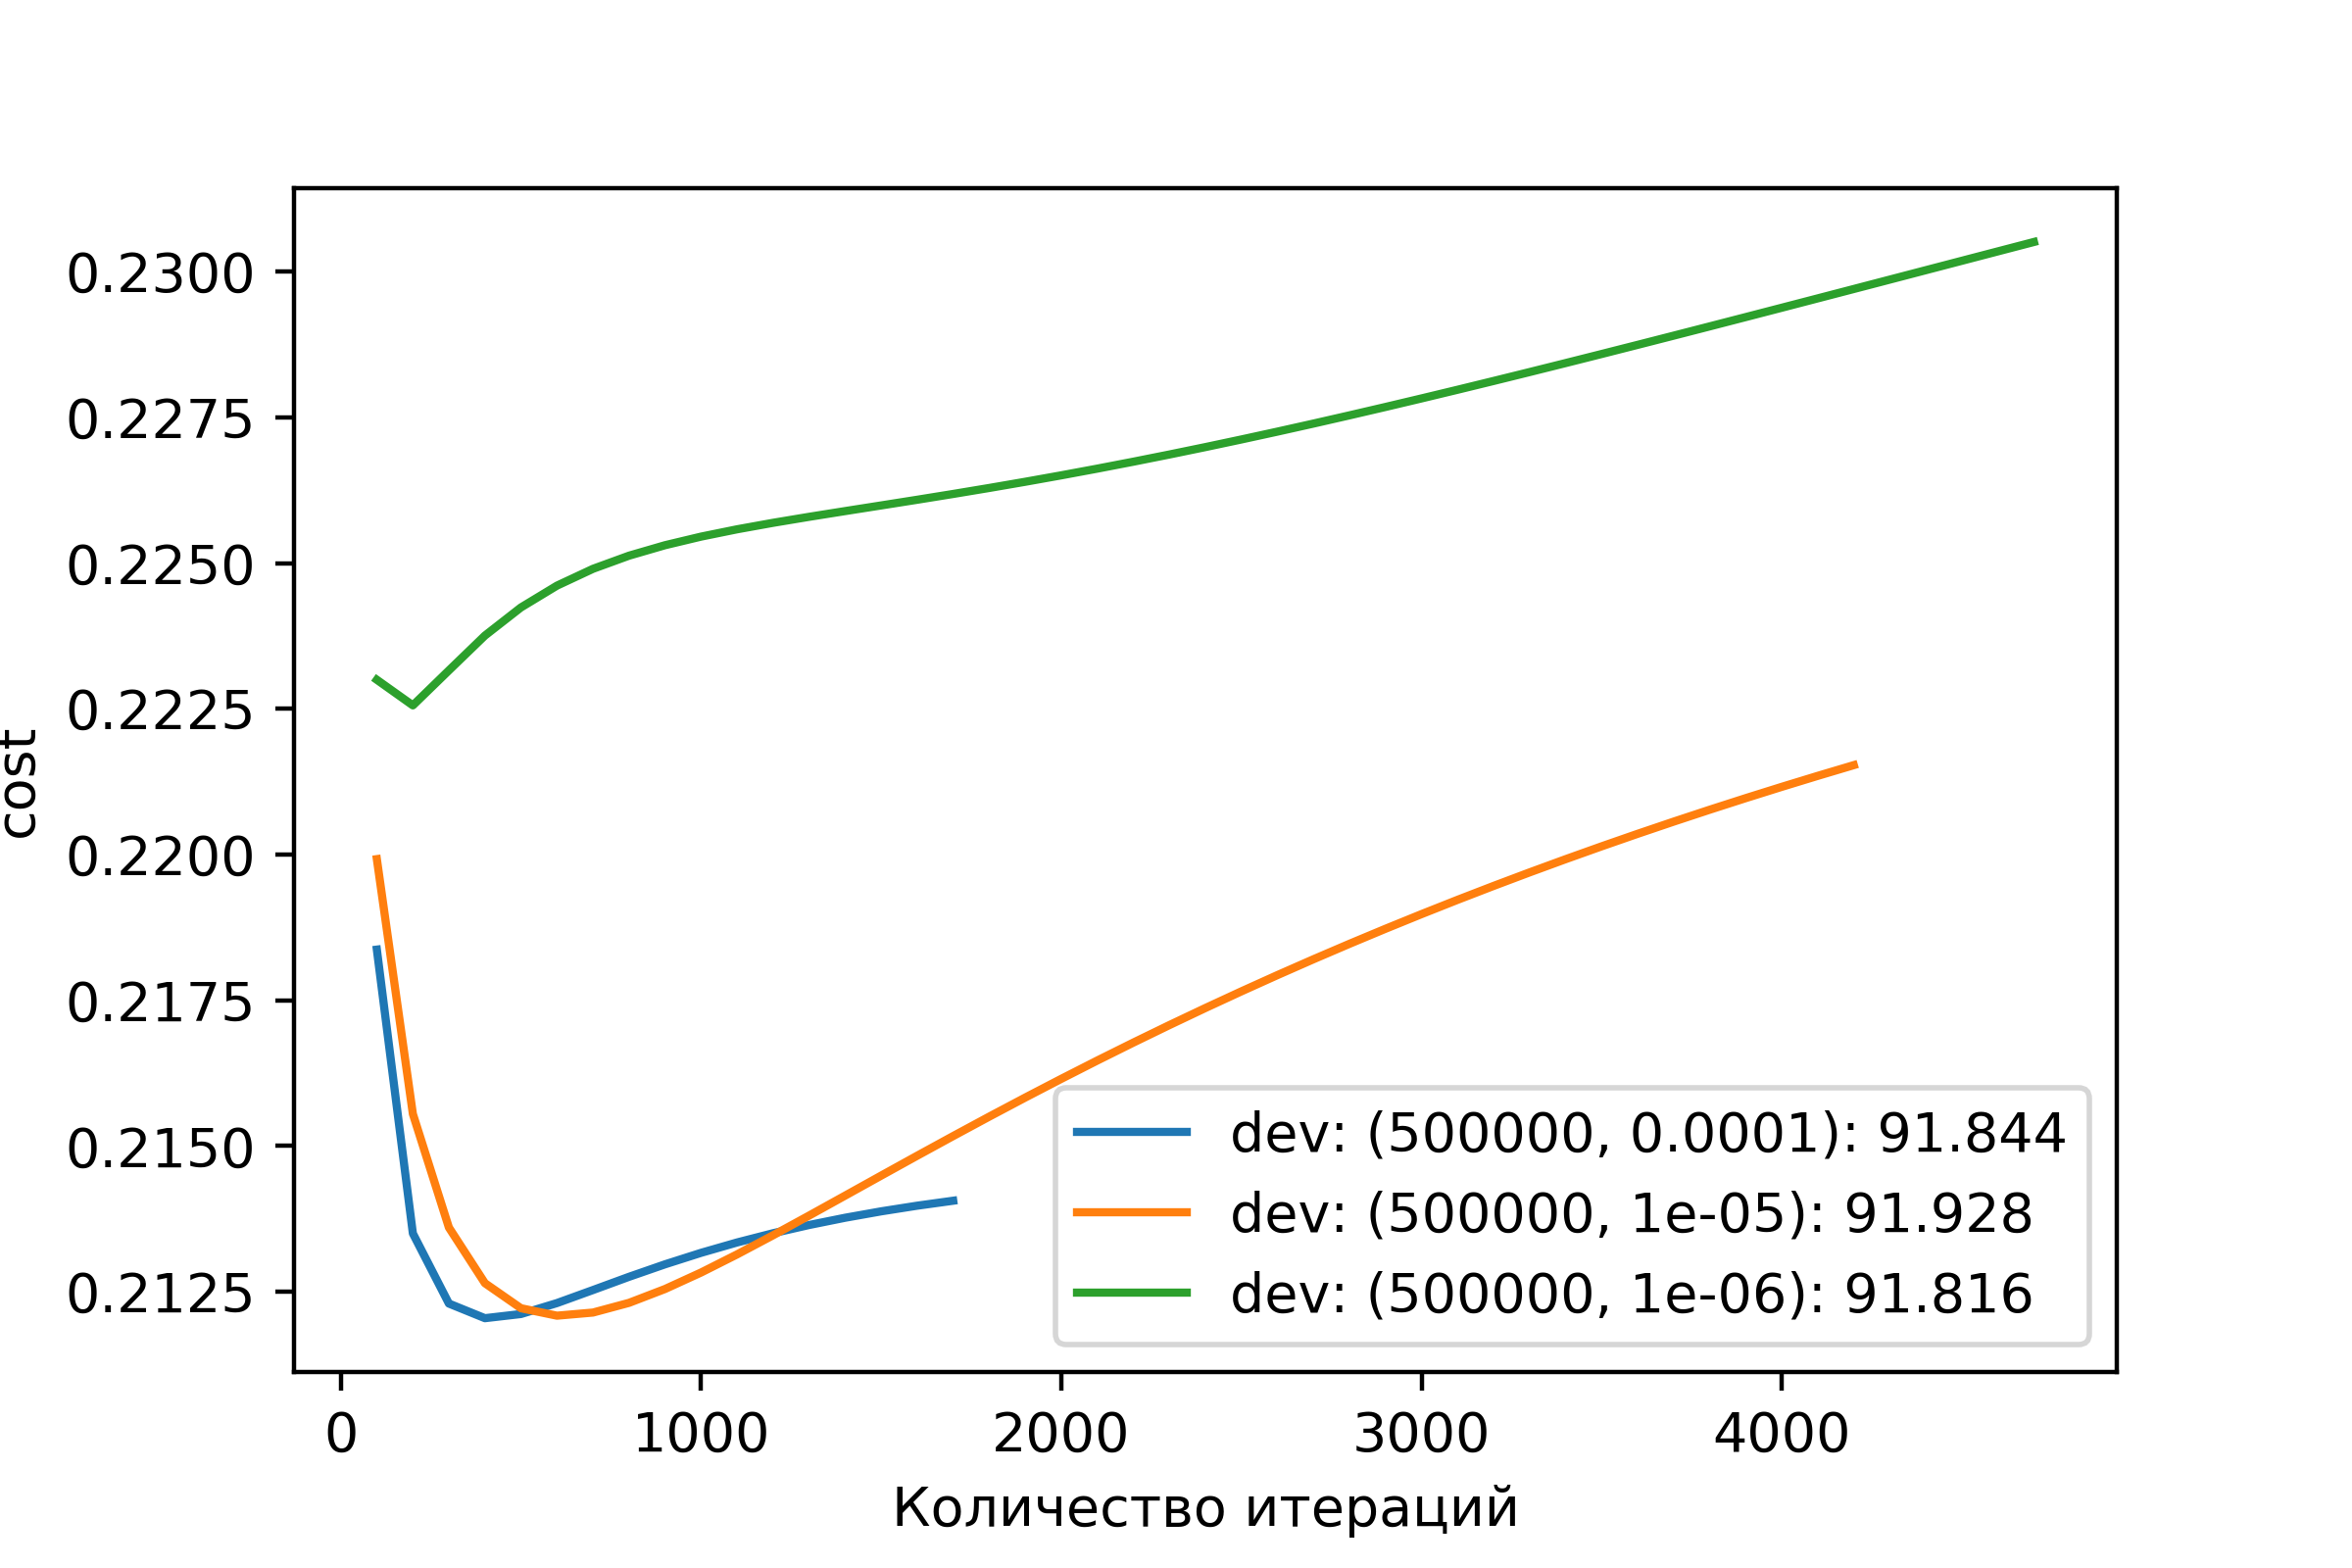
\includegraphics[width=0.5\textwidth, height=0.4\textwidth]{3g_weight_500000.png}
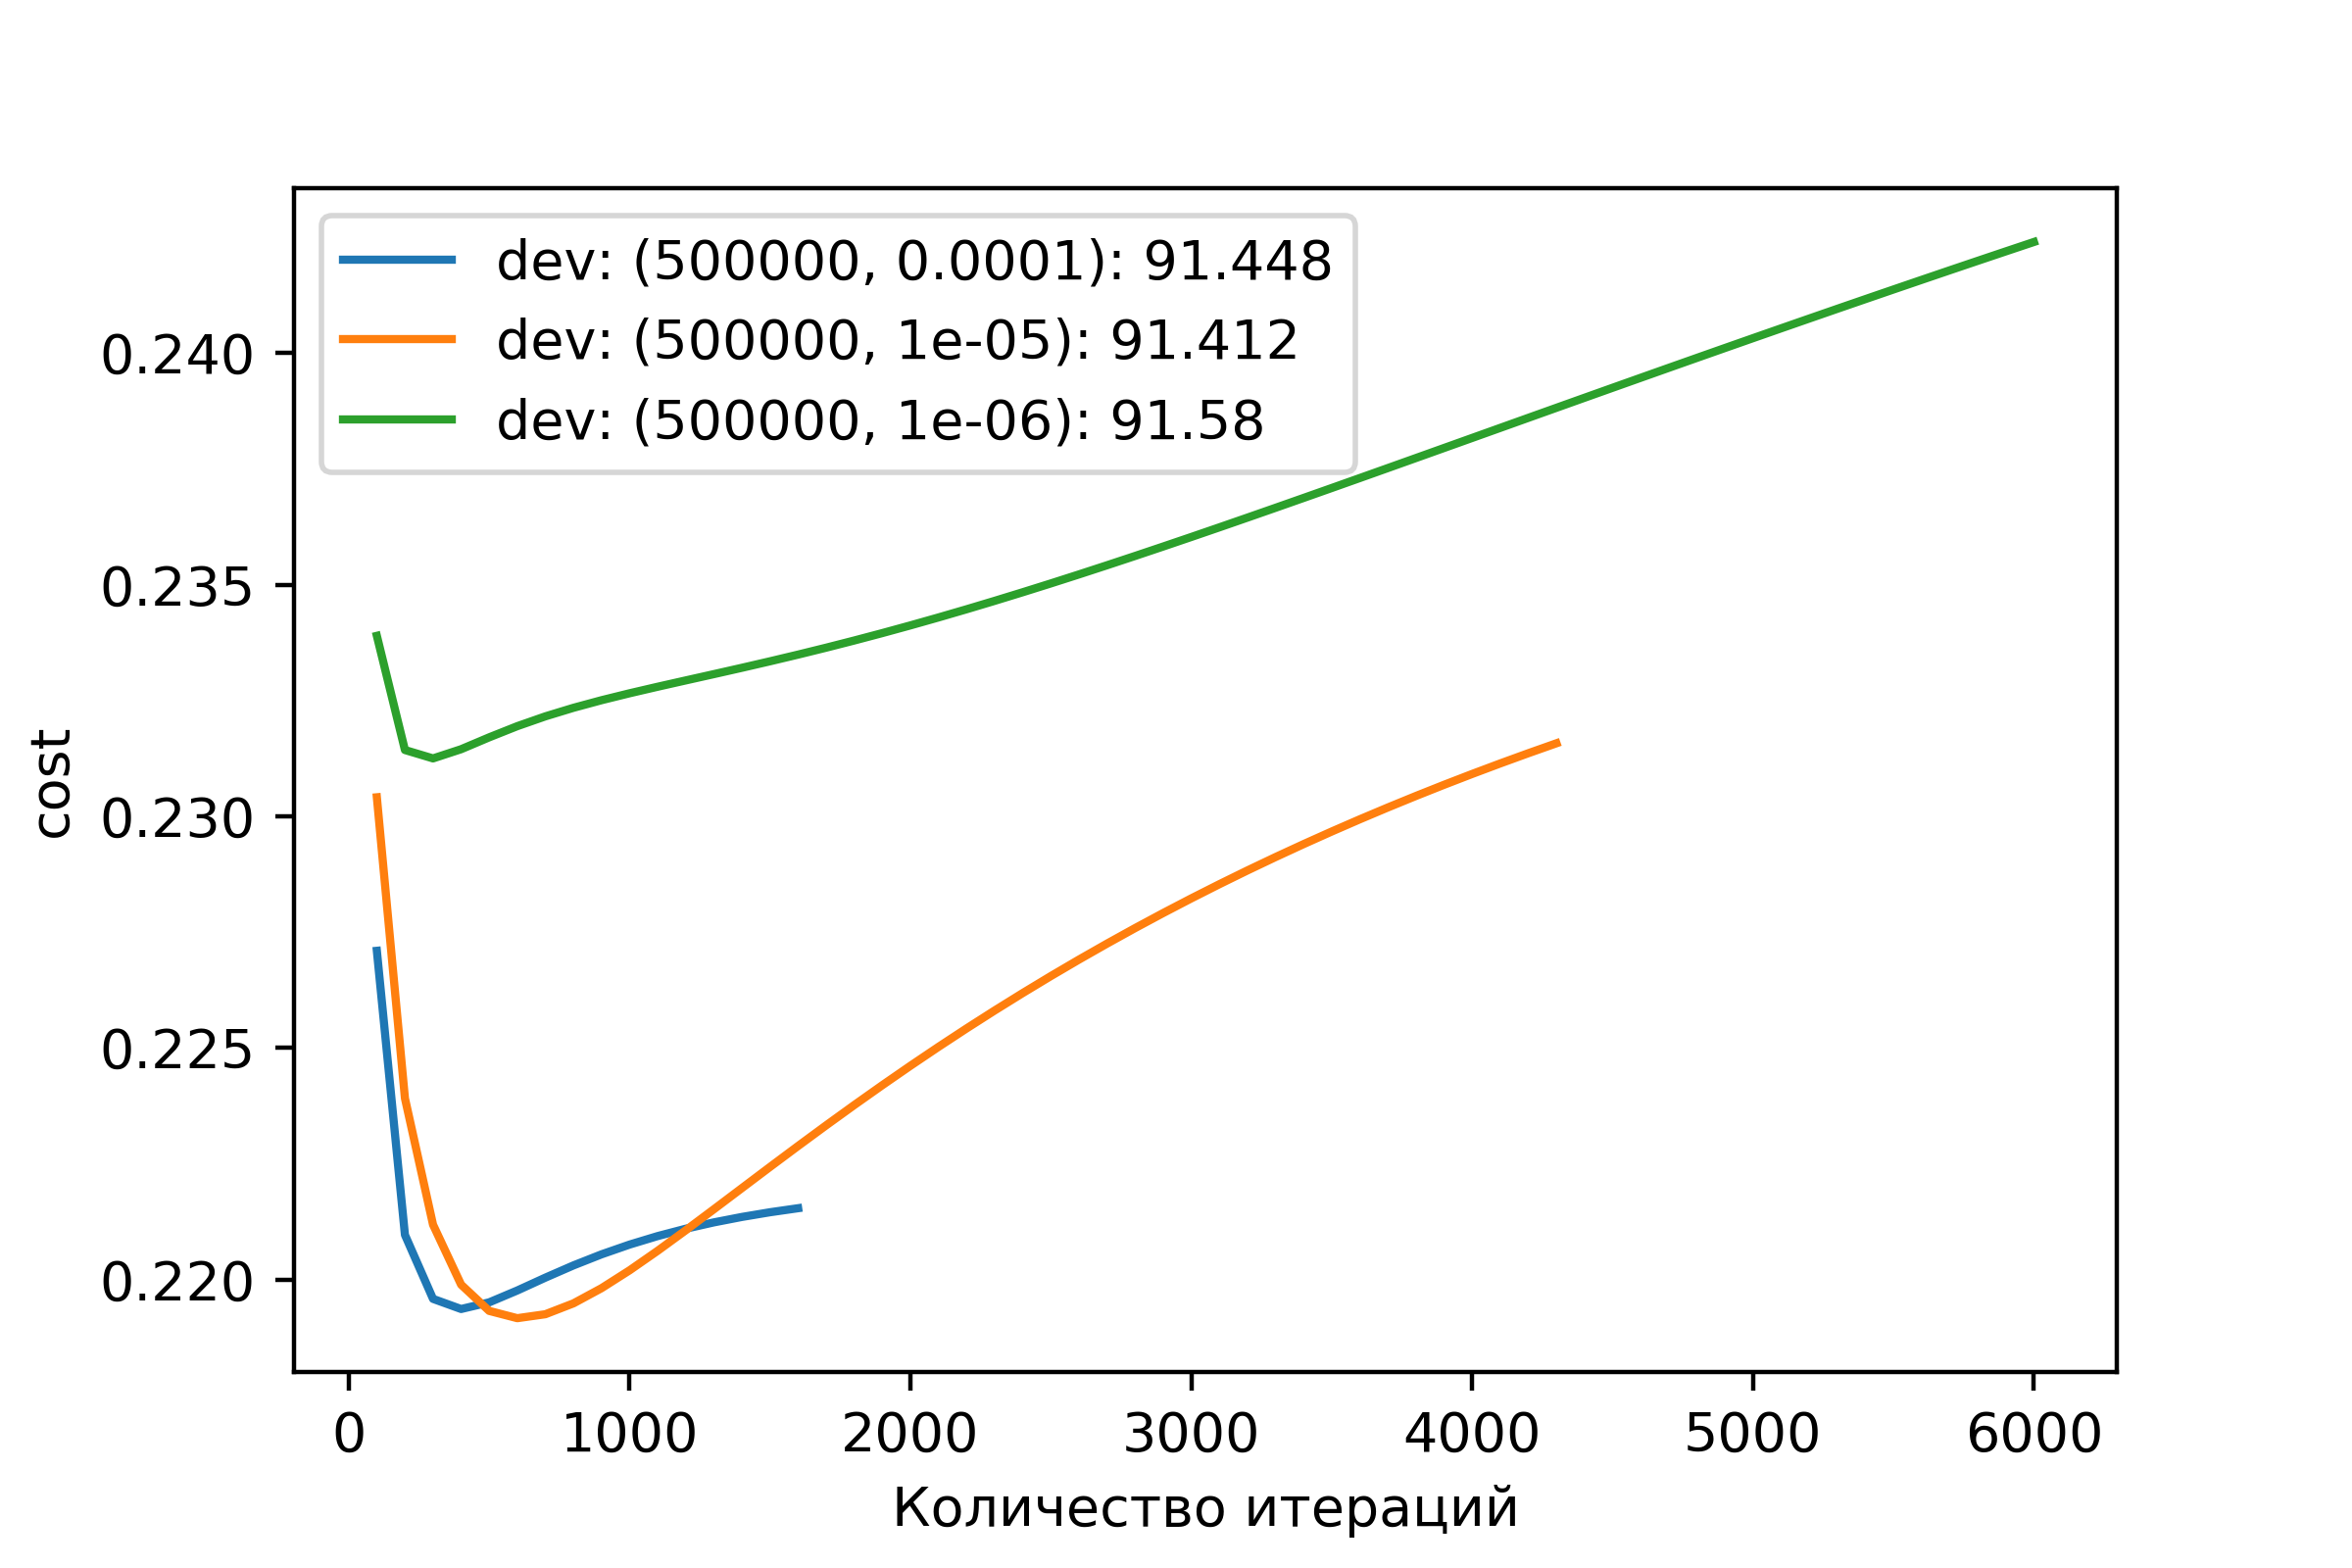
\includegraphics[width=0.5\textwidth, height=0.4\textwidth]{2g_weight_500000.png}\\
\caption{Зависимость функции ошибок от количества итераций в ходе оптимизации параметров модели для 3g (слева) и 2g (справа) с применением взвешивания}
\label{3+2grams:weighted}
\end{figure}

\begin{figure}
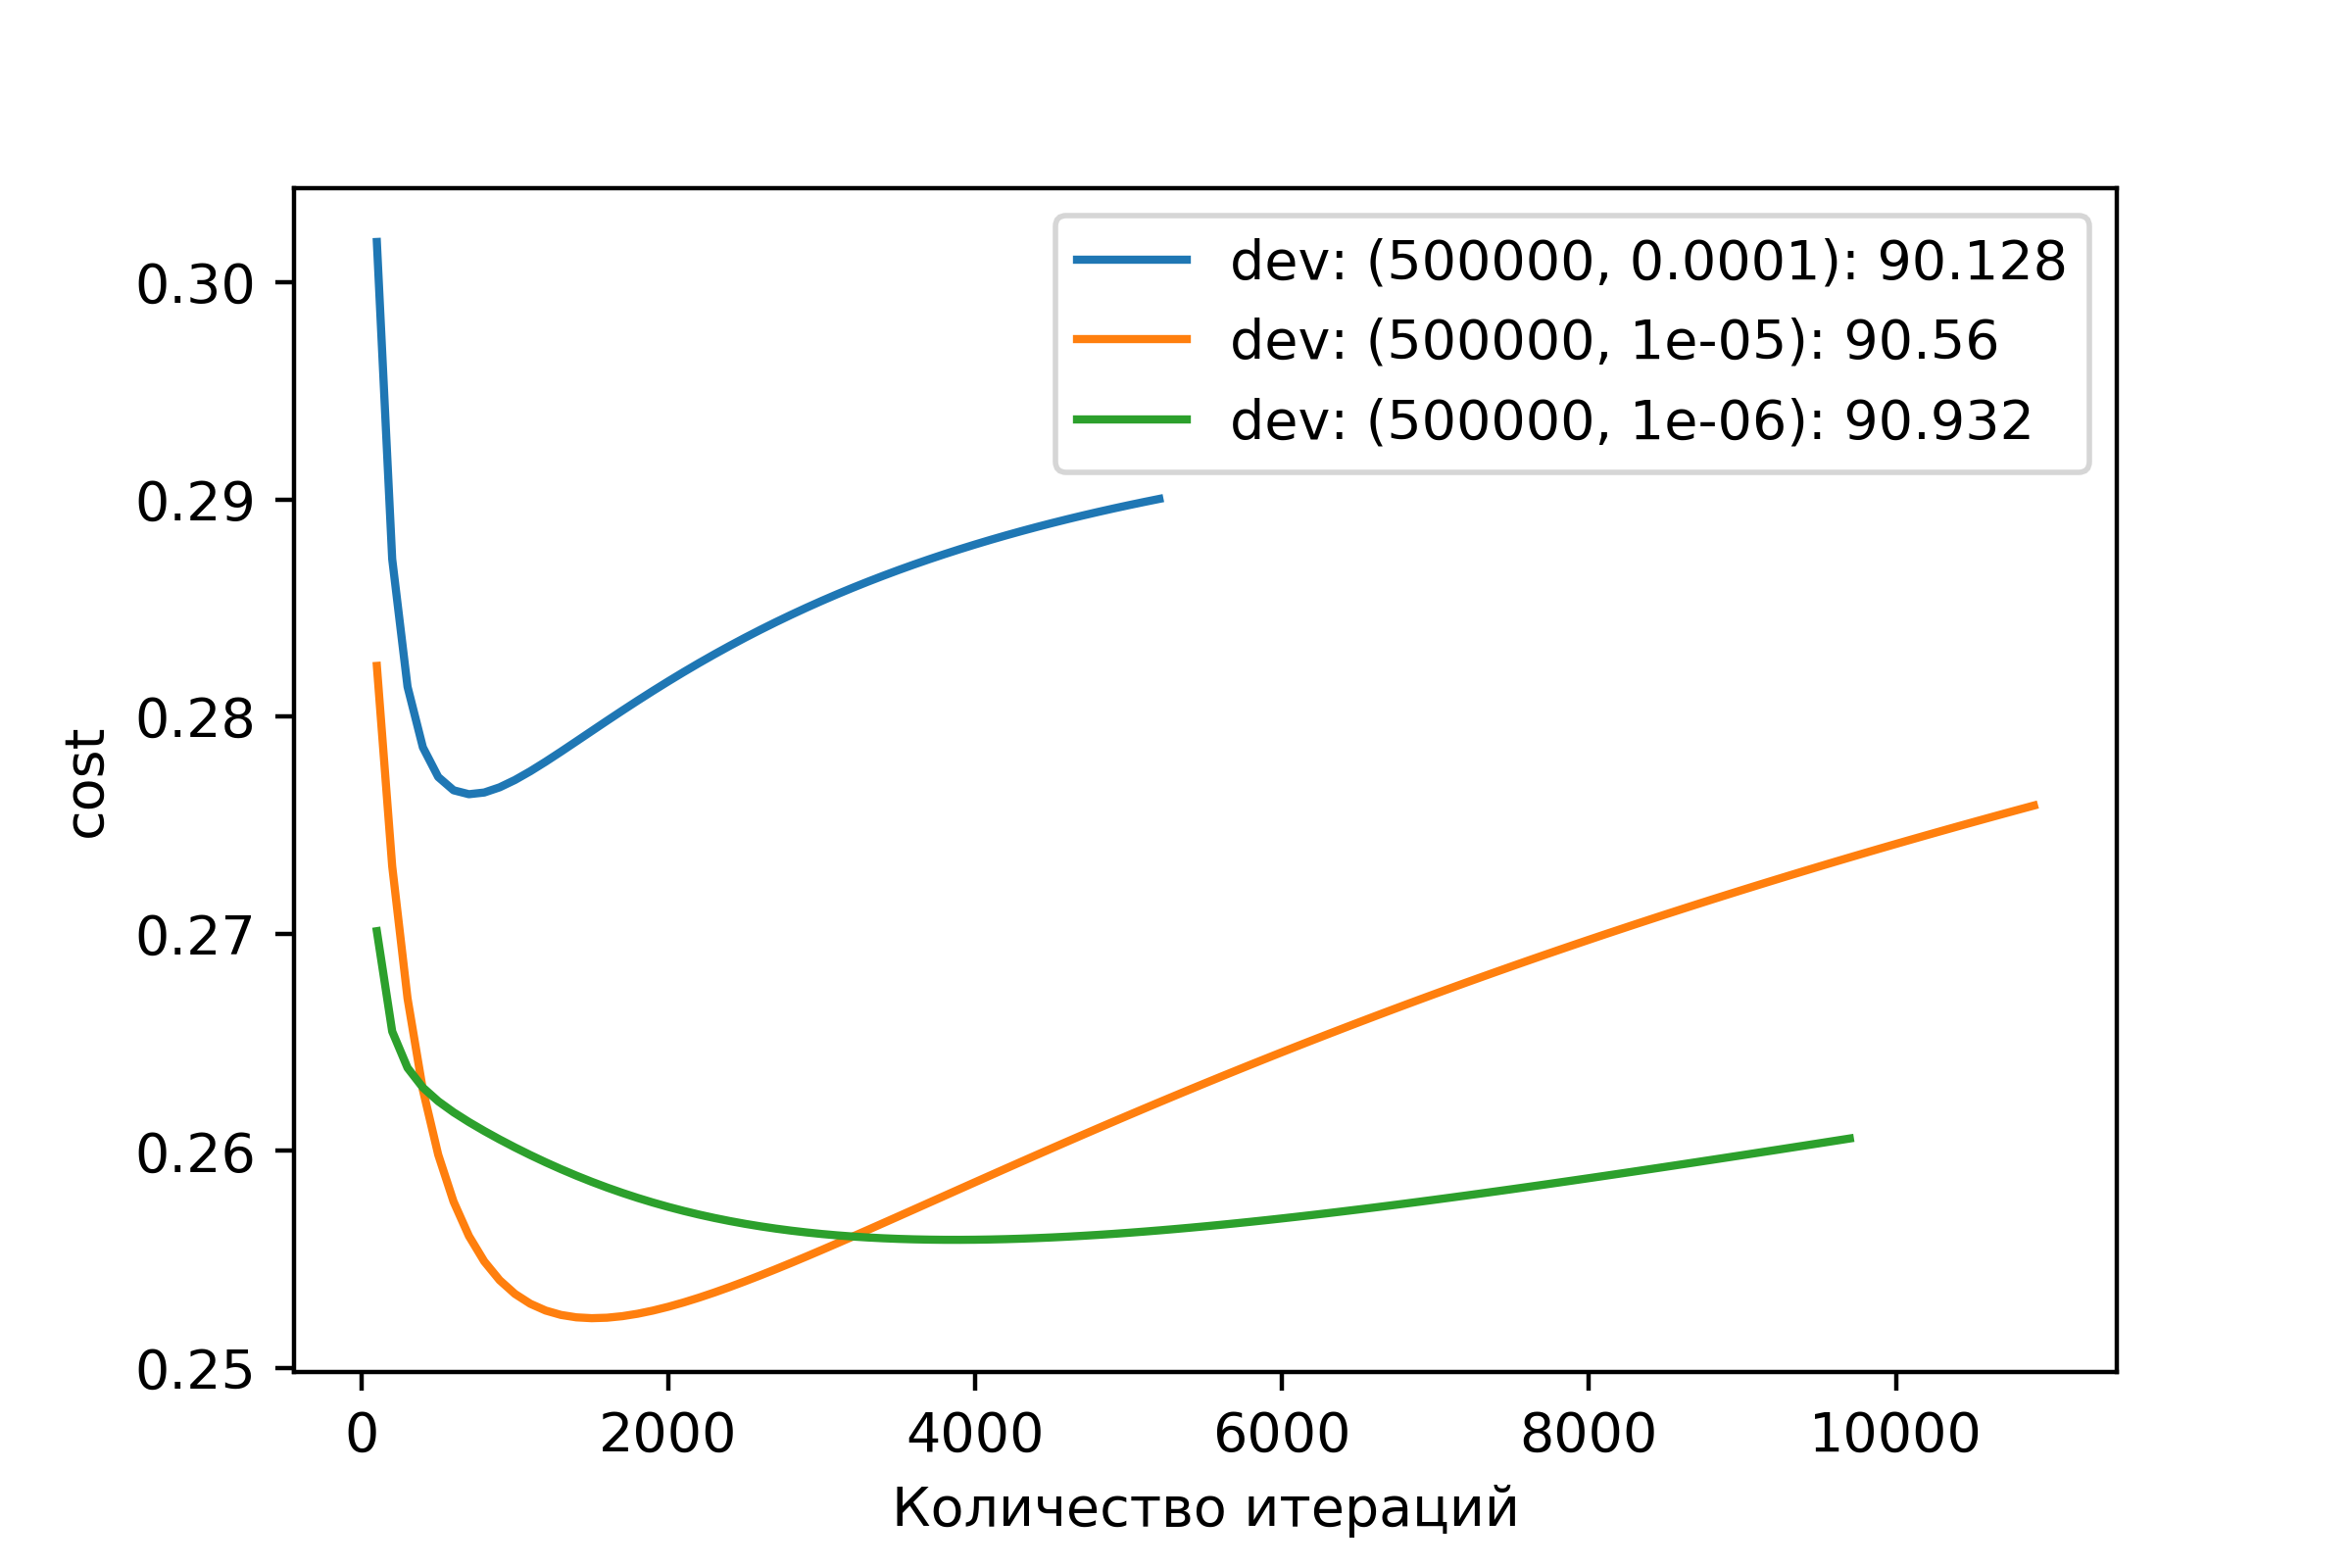
\includegraphics[width=0.5\textwidth, height=0.4\textwidth]{2g_def_500000.png}
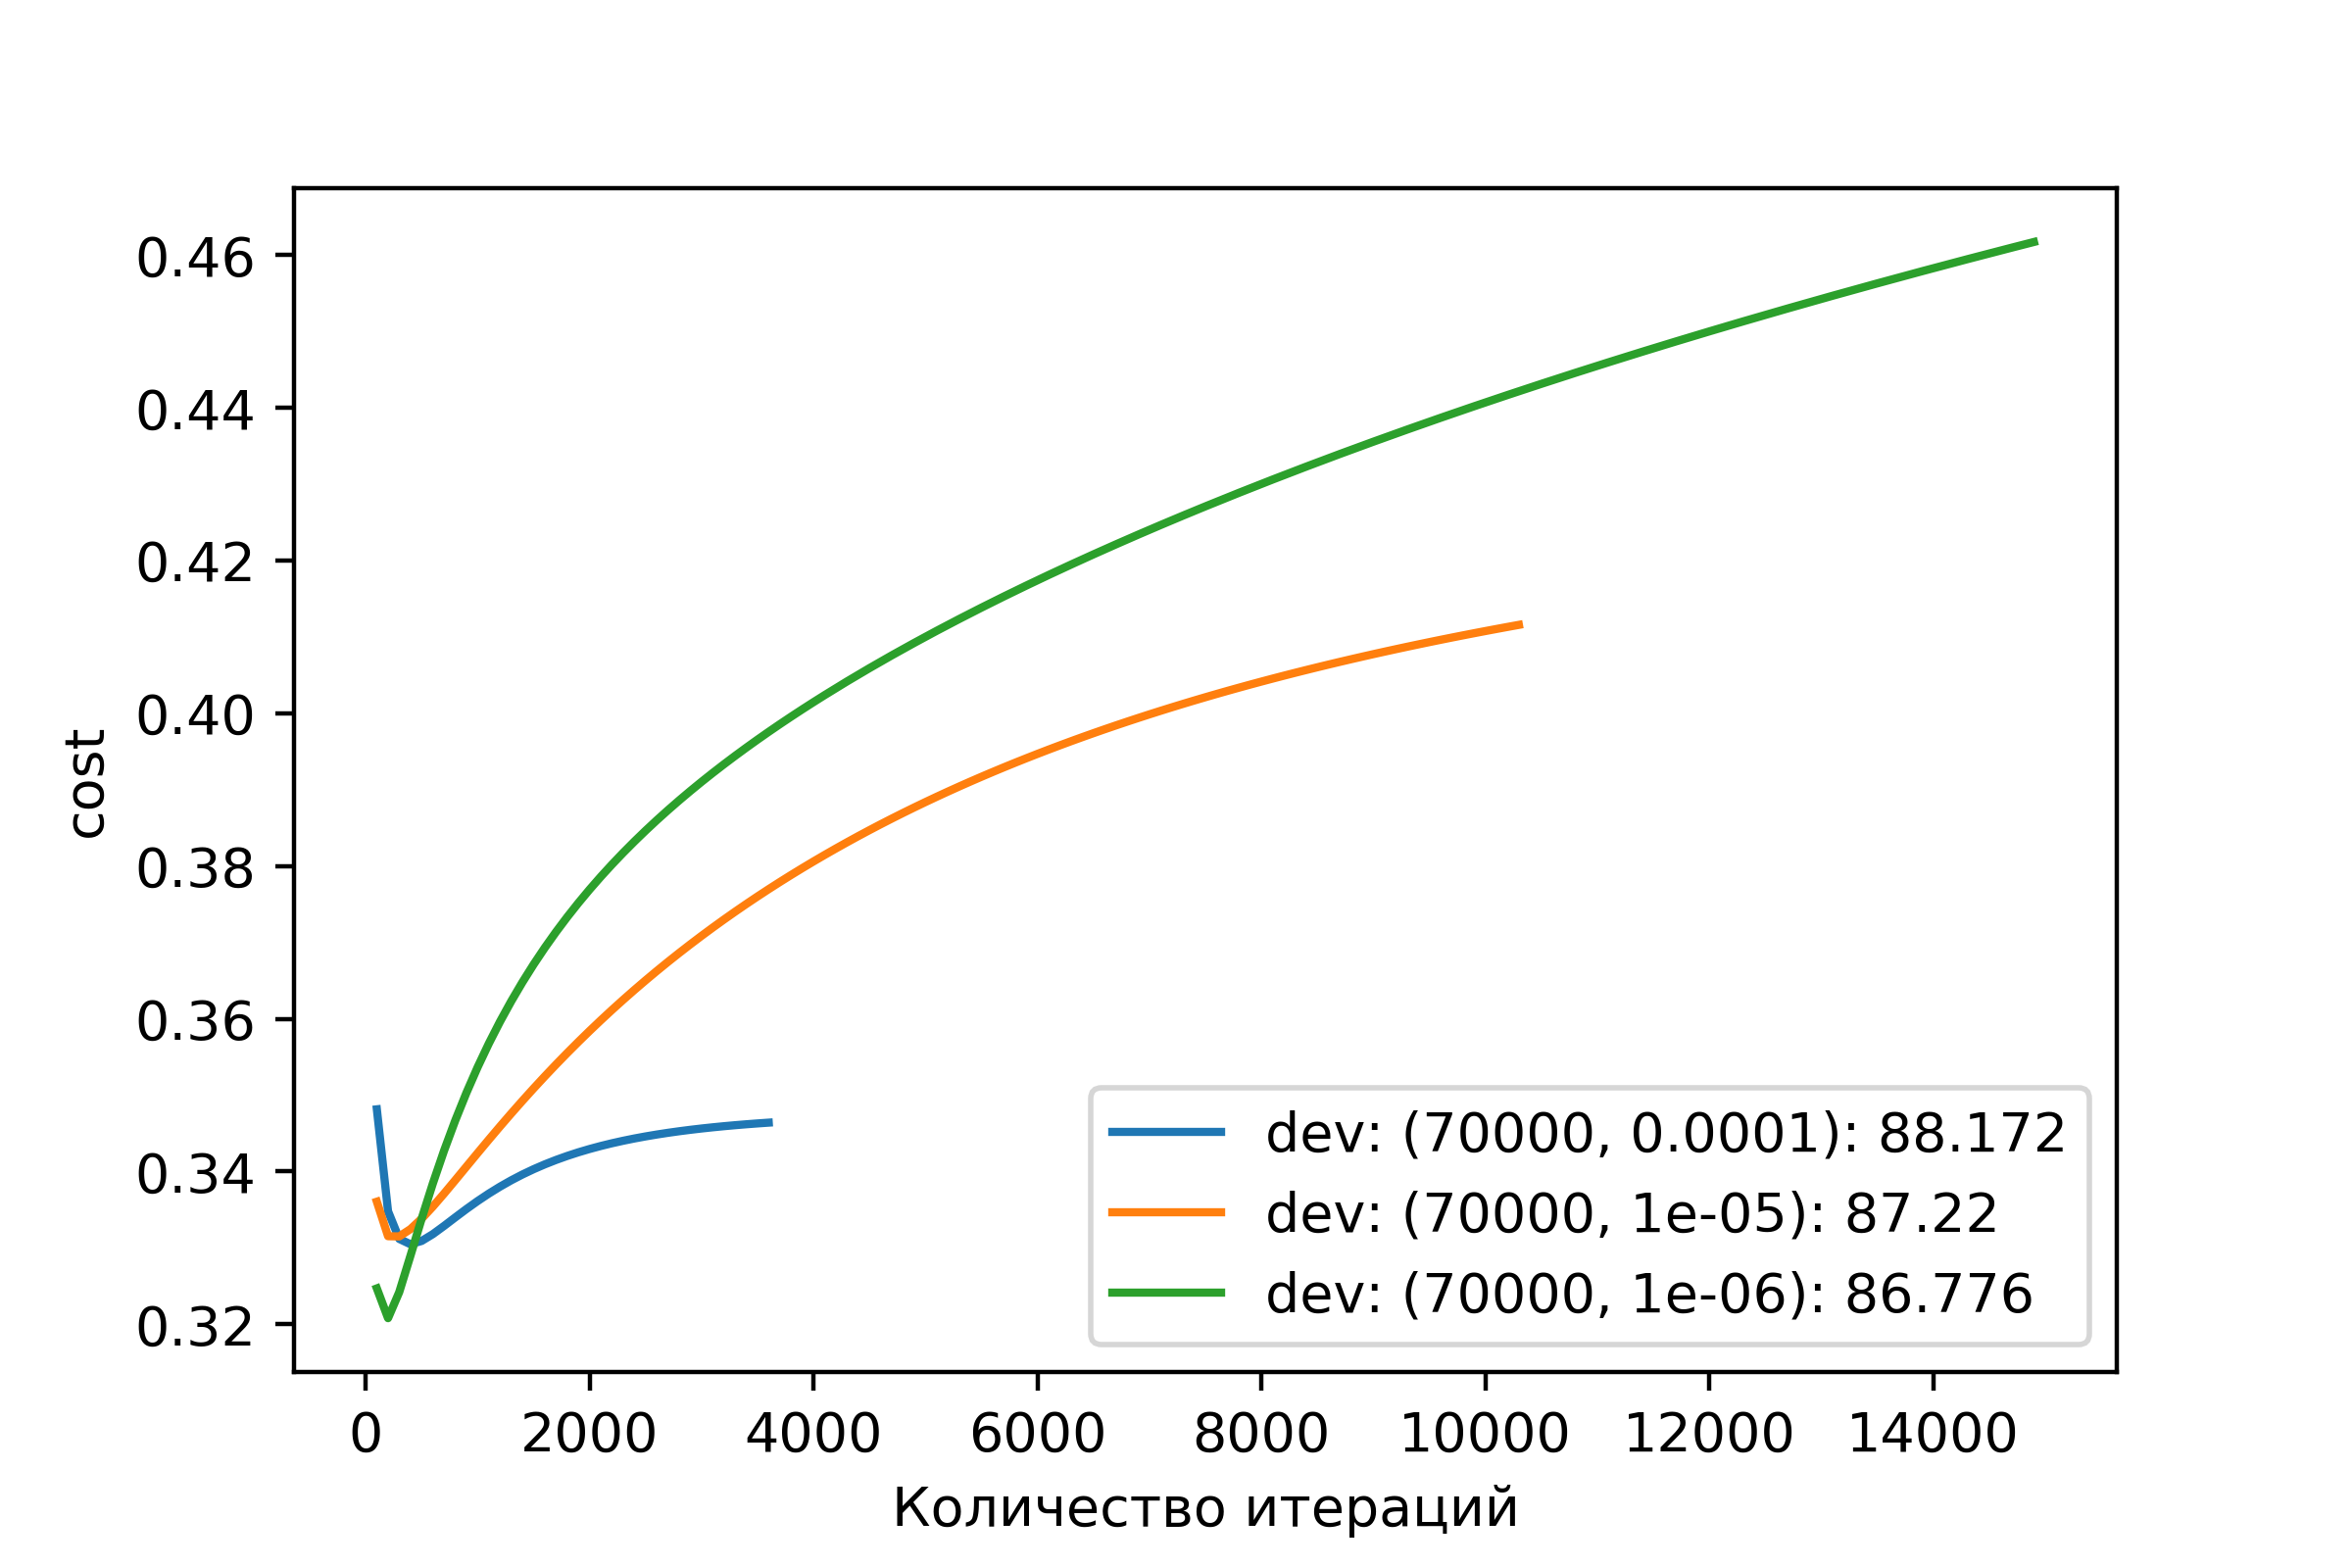
\includegraphics[width=0.5\textwidth, height=0.4\textwidth]{1g_def_70000.png}\\
\caption{Зависимость функции ошибок от количества итераций в ходе оптимизации параметров модели для 2g (слева) и униграммов (справа) без применения взвешивания}
\label{3+2grams:default}
\end{figure}
\subsection{Результаты}
В таблице\,\ref{logistic:results} приведены результаты проведенных экспериментов. В ходе экспериментов нам удалось улучшить результат указанный в \cite{ensemble:GregoireMesnil} для линейной модели. Также улучшили результат из \cite{Narayanan:naiveBayes} для наивного байесовского классификатора.

Для задач анализа тональности текста логистическая регрессия работает значительно лучше наивного байесовского классификатора. Как мы видим, отрыв составляет порядка 2\%.

Как видно из таблицы, при взвешивании признаков результат увеличивается примерно на процент. При добавлении триграмма рост точности составляет половину процента. При включении еще и четыреграммов, нам удалось получить результат 92.076 для логистической регрессии со взвешиванием признаков.

\section{Ошибки}
Рассматриваются модели логистической регрессии после обучения с N-граммами до триграммов включительно, размером словаря равным 500000 и коэффициентом регуляризации равным $1e-05$ с применением взвешивания и без него.

В модели со взвешиванием признаков было допущено 2018 ошибок, причем количество неправильно классифицированных положительных отзывов составляет 998, а отрицательных 1020.

Во второй модели ошибок всего 2272, неверно классифицированных положительных отзывов 1107, отрицательных же 1165.

Как видно, в обеих моделях допускается примерно одинаковое количество ошибок в положительных и отрицательных отзывах.

Примеры текстов с ошибками классификации с применением взвешивания представленны в таблице \ref{logistic:examples}.
\begin{table}
\begin{tabular*}{\textwidth}{p{0.65\textwidth} @{\extracolsep {\fill}} ccc}
\hline {\bf Отзыв} & {\bf Увер.} & {\bf Отв.} & {\bf Знач.} \\ \hline \hline
{1. A really realistic, sensible movie by Ramgopal Verma . No stupidity like songs as in other Hindi movies. Class acting by Nana Patekar. <br /><br />Much similarities to real 'encounters'.} & -0.088 & \colorbox{pink}{neg} & \colorbox{lime}{pos} \\ \hline
{2. It's not Citizen Kane, but it does deliver. Cleavage, and lots of it.<br /><br />Badly acted and directed, poorly scripted. Who cares? I didn't watch it for the dialog.} & -2.25 & \colorbox{pink}{neg} & \colorbox{lime}{pos} \\ \hline
{3. I don't care if some people voted this movie to be bad. If you want the Truth this is a Very Good Movie! It has every thing a movie should have. You really should Get this one.} & -0.764 & \colorbox{pink}{neg} & \colorbox{lime}{pos} \\ \hline
{4. The plot was really weak and confused. This is a true Oprah flick. (In Oprah's world, all men are evil and all women are victims.)} & 0.278 & \colorbox{lime}{pos} & \colorbox{pink}{neg} \\ \hline
{5. Masterpiece. Carrot Top blows the screen away. Never has one movie captured the essence of the human spirit quite like Chairman of the Board. 10/10... don't miss this instant classic.} & 4.007 & \colorbox{lime}{pos} & \colorbox{pink}{neg} \\ \hline
{6. A dedicated Russian Scientist dreams of going to Mars. He eventually gets there but it takes the whole film before we are able to have a laugh at the Russian style of Revolution in Mars.} & 0.157 & \colorbox{lime}{pos} & \colorbox{pink}{neg} \\ \hline
\end{tabular*}

\caption{Примеры ошибок при классификации обученной моделью логистической регрессиии со взвешиванием признаков}
\label{logistic:examples}
\end{table}
\section{Признаки моделей}
В таблице \ref{features} приводятся по 20 признаков для моделей логистической регрессии со взвешиванием и без взвешивания, на которые они опираются при классификации. Можно видеть, что есть признаки, сильно влияющие результат и присутствующие в обеих моделях.

\begin{table}
\begin{tabular*}{\textwidth}{c @{\extracolsep {\fill}} ccc}
\hline \multicolumn{2}{c}{Модель со взвешиванием} & \multicolumn{2}{c}{Модель без взвешивания} \\ \hline
Положительные & Отрицательные & Положительные & Отрицательные \\
признаки & признаки & признаки & признаки \\ \hline \hline
and does & see why & attention & see why \\ \hline
a trip & 4 10 & and does & if you have \\ \hline
the extreme & released and & the worst & green \\ \hline
was interesting & dawson & otherwise & couple \\ \hline
true life & the cabin & many other & fun \\ \hline
needed a & the jokes & a trip & all of \\ \hline
save the day & slater & the extreme & stand \\ \hline
was happening & dr hackenstein & was interesting & i like \\ \hline
perception & worst acting & you have a & people are \\ \hline
not appear & profession & bobby & she doesn \\ \hline
beginning of this & everything you & what a & movie was \\ \hline
him how & tara reid & human & the jokes \\ \hline
you have a & shaggy & maybe it & playing \\ \hline
leno & blazing & like this & i never \\ \hline
many other & programs & bad guys & 4 10 \\ \hline
s set & roman & the american & help \\ \hline
so obvious & burn it & ratings & acting was \\ \hline
only complaint & binder & sound & all of the \\ \hline
criticisms & traffic & was in & but even \\ \hline
acting in & she doesn & edge & killer \\ \hline
\end{tabular*}
\caption{Ниболее важные признаки, на которые опираются модели при классификации в порядке убывания}
\label{features}
\end{table}